\section{Results}\label{results}
In this section we will describe our results both locally against our self and
against two other groups in a tournament setting.

\subsection{Local}\label{results:local}
One of the first things we wanted to know when we had created our minimax 
implementation is when we should switch. As the first few positions have very
little bearing on the rest of the game, we can play a few moves as a novice
before switching to the minimax algorithm. To test when this switch should
occur we played our minimax algorithm against it self in a number of scenarios
to see when we should switch. 

\begin{figure}[htb]
	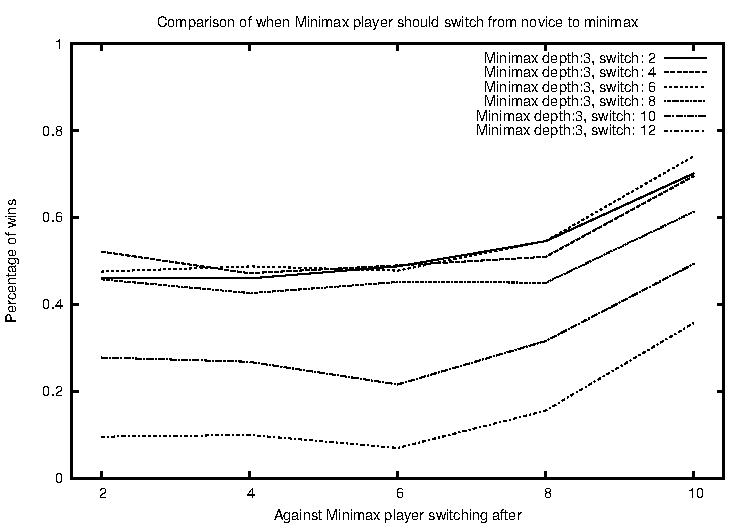
\includegraphics{graphs/switch.pdf}
	\caption[Minimax switch graph]{Graph describing our minimax switch results}
	\label{fig:minimax switch}
\end{figure}

We ran the code in listing \ref{lst:switch code} and got the results you can see in figure
\ref{fig:minimax switch}. From this we can see that switching on 2, 4 and 6 is 
really not any different.
The small difference we can see is just random variance because of the single
run we have tested. When we get down to switching after 8 pieces has been placed
there is some difference and we start to see a drop in efficiency.

\subsection{Tournament}\label{results:tournament}


%TODO: there needs to be more text here
